% Created 2024-12-09 Mo 14:43
% Intended LaTeX compiler: lualatex
\documentclass{mimosis}
                  \usepackage[hyperref,x11names]{xcolor}
\usepackage[
colorlinks = true,
citecolor  = RoyalBlue,
linkcolor  = RoyalBlue,
urlcolor   = RoyalBlue,
unicode
]{hyperref}
\usepackage{fontspec}
\usepackage{ltablex}
\usepackage{unicode-math}
\setmonofont{DejaVu Sans Mono}[Scale=0.8]
\newenvironment{abstract} {}{}
\usepackage{abstract}
\DeclareMathOperator*{\argmax}{arg\,\max}

%% ox-latex features:
%   !announce-start, bibliography-biblatex, !guess-pollyglossia, !guess-babel,
%   !guess-inputenc, caption, image, bibliography-biblatex-resources,
%   !announce-end.

\usepackage{biblatex}


\usepackage{capt-of}

\usepackage{graphicx}

\addbibresource{~/org/resources/bibliography/refs.bib}

%% end ox-latex features

\author{ProceduralTree}
\date{\today}
\title{Project Thesis}
\hypersetup{
 pdfauthor={ProceduralTree},
 pdftitle={Project Thesis},
 pdfkeywords={},
 pdfsubject={},
 pdfcreator={Emacs 29.4 (Org mode 9.8-pre)}, 
 pdflang={English}}
\begin{document}

\maketitle
\setcounter{tocdepth}{1}
\tableofcontents

\begin{abstract}
This work shows sensitivity of boundary conditions for two different finite difference approaches to solving the Cahn-Hilliard equation
\end{abstract}
\chapter{Introduction}
\label{sec:orgb38f6a5}
This project thesis builds upon the work in our bachelor thesis, by introducing a simple boundary condition approach to a variation of the solver used therein. In Chapter \ref{sec:org755846c} we introduce the Cahn-Hilliard equation in the formulation that we use for this project. This project used a two-dimensional second order version of this CH equation rather than the usual 1D 4th order one, to simplify the numerical implementation. The solver itself builds upon a finite difference discretization of this equation. In Chapter \ref{sec:orgeeaed4d}, together with the discrete domains, on which we run our numerical solver, we introduce a Jacoby iteration to solve the linear system derived from the aforementioned discretization.  The numerical solver in this thesis is GPU accelerated, and the discretization we chose to base our solver on is capable to calculate on all domains as long as a characteristic function is given. Therefore, we introduce two domains, on which we present our findings. The primary goal of this work is then the boundary condition approach in Chapter \ref{sec:orgb84ef3a}. Conceptionally the boundary condition we introduce simply consists of a constant value added in the linear system to all equations corresponding to grid-cells on the boundary. The actual implementation is capable of doing this for arbitrary domains. We present the results of this method on two Domains, a square one in \ref{sec:orgb47f456} and a circular domain in \ref{sec:org8f4cb79} where we show the phase field for different boundary conditions which manifest in a variable contact angle of the interface on the boundary mimicking the behavior of hydrophobic/hydrophilic material. While we are unable to provide explicit formulae in relation to the constant, in Chapter \ref{sec:org214e230} we provide numerical insight in this relationship, and a table with precomputed values.
\chapter{Fundamentals}
\label{sec:org755846c}
This work concerns itself with boundary conditions on the CH equation. The CH equation is a fourth order differential equation that provides a phasefield \(\phi\) which is used for implicit interface formulation. The Cahn Hilliard equation, in the formulaton we use here, is derived from the \textbf{Ginzburg-Landau} energy, an example on how this is done is given by \autocite{Wu_2022}.
\begin{align}
\label{eq:energy}
E^{\text{bulk}}[\phi] &= \int_{\Omega} \frac{\varepsilon^2}{2} |\nabla \phi |^2 + W(\phi) \, dx ,
\end{align}
There they introduce a chemical potential \(\mu\) derived as derivative of the \textbf{Ginzburg-Landay} energy.
\begin{align}
\label{eq:chemical-potential}
 \mu &= \frac{\delta E_{bulk}(\phi)}{\delta \phi} = -\varepsilon^2 \Delta \phi + W'(\phi)
\end{align}
where \(W(\phi)\) in the energy,is a double well potential. In our case we orient us at the work of\autocite{SHIN20117441}, where they use
\begin{equation}
\label{eq:6}
W(\phi) = \frac{(1-\phi^2)^2}{4}.
\end{equation}
they Cahn Hilliard equation in this thesis is then given as
\begin{equation}
\begin{aligned}
\partial_{t}\phi(x,t) &=  \Delta\mu \\
\mu &= - \varepsilon^2 \Delta\phi  + W'(\phi).
\end{aligned}
\end{equation}
one thing to note is, that this way of writing the CH equation is secend order two dimensional rather than the one dimensional fourth order often given.
\begin{equation}
\label{eq:7}
\partial_t \phi(\vec{x} , t) = - \Delta(\varepsilon^2  \Delta \phi + W\prime(\phi))
\end{equation}
this choice is deliberate, and aligns with the numerical implementation.
\section{Notation}
\label{sec:orgc5a0896}
This project solves the CH equation on a regular rectangular grid with grid-size \(h\). The computational domain, is therefore discretized as
\begin{align}
\label{eq:4}
\vec{x}_{ij} &:= \frac{i}{h} * e_{1} + \frac{j}{h} e_2
\end{align}
We then write the discrete fields
\begin{align}
\label{eq:5}
\phi_{ij}^n &: \Omega_d \times \left\{ 0, \dots  \right\} \to \mathbb{R} \,,\\
\phi_{ij} &:= \phi(\vec{x}_{ij}) & \vec{x}_{ij} \in \Omega_{d} \\
\mu_{ij}^n &: \Omega_d \times \left\{ 0, \dots \right\} \to \mathbb{R} \,, \\
\mu_{ij} &:= \mu(\vec{x}_{ij})
\end{align}
We use the following differential quotients:
\begin{align}
D_xf_{i+\frac{1}{2} j} &= \frac{f_{i+1j} - f_{ij}}{h} & D_yf_{ij+\frac{1}{2}} &= \frac{f_{ij+1} - f_{ij}}{h}
\end{align}
And define a discrete gradient as.
\begin{equation}
\nabla_d f_{ij} = (D_x f_{i+1j} , \ D_y f_{ij+1})
\end{equation}
See \autocite{Ulmer_CHRelaxed_2024}
\chapter{Boundary adaptation}
\label{sec:orgb84ef3a}
The solver we use as reference guaranties no flux boundary conditions at a discrete level by setting \(\nabla \phi_{ij} = 0\) for \(\phi_{ij} \in \partial \Omega_{d}\) this is done by multiplying with the Characteristic function of \(\Omega_{d}\)
\begin{equation}
G_{ij}=
\begin{cases}
1 \,, x_{ij} \in \Omega \\
0 \,, x_{ij} \not\in \Omega \\
\end{cases}
\end{equation}
To accommodate different boundary conditions, we bias \(\nabla_d \cdot (G_{ij} \nabla_d \phi_{ij})\) in grid points next to the boundary. We determine those points using a centered difference scheme on \(G\)
\begin{equation}
B_{ij} = \max\left(  |G_{i+\frac{1}{2}j} - G_{i-\frac{1}{2}j}| , |G_{ij+\frac{1}{2}} - G_{ij-\frac{1}{2}}|\right) * C
\end{equation}
Where \(C\) is a constant we chose freely. For example on a 32x32 Domain with \(C=1\) the Boundary field \(\mathbf{B}\) appears as follows


\begin{figure}[htbp]
\centering
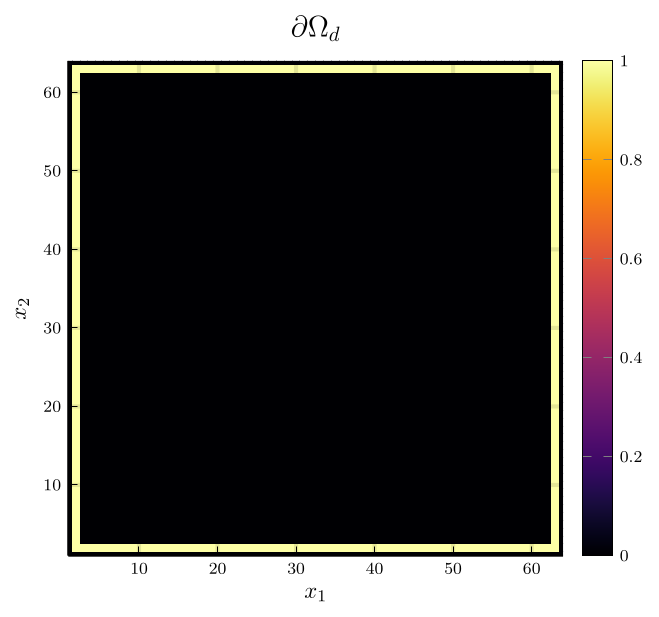
\includegraphics[width=.9\linewidth]{images/boundary.png}
\caption{\label{fig:boundary-square}visualization of all grid-cells adjacent to the boundary \(\partial \Omega_{d}\) of a square domain}
\end{figure}

\begin{figure}[htbp]
\centering
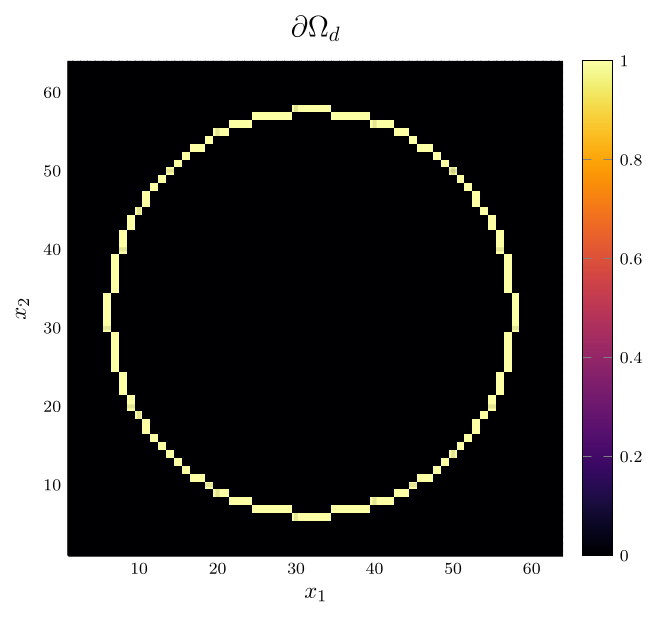
\includegraphics[width=.9\linewidth]{images/boundary-circle.png}
\caption{\label{fig:boundary-circle}visualization of all grid-cells adjacent to the boundary \(\partial \Omega_{d}\) of a circular domain}
\end{figure}



We then state the adapted approach as:
\begin{equation}
\label{eq:second-order-adapted-ansatz}
\begin{aligned}
\frac{\phi_{ij}^{n+1} - \phi_{ij}n}{\Delta t}  &=  \nabla _d \cdot (G_{ij} \nabla_d \mu_{ij}^{n+\frac{1}{2}} )  \\
 \mu_{ij}^{n+\frac{1}{2}} &= 2\phi_{ij}^{n+1} - \varepsilon^2  \nabla_d \cdot  (G_{ij} \nabla _d \phi_{ij}^{n+1} ) + B_{ij} + W'(\phi_{ij}^n) - 2\phi _{ij}^n
\end{aligned}
\end{equation}

*Furthermore, our solver implements the ansatz proposed by the authors \autocite{SHIN20117441}.
\begin{equation}
\label{eq:ansatz}
\begin{aligned}
\frac{\phi_{ij}^{n+1} - \phi_{ij}^n}{\Delta t}  &=  \nabla _d \cdot (G_{ij} \nabla_d \mu_{ij}^{n+\frac{1}{2}} )  \\
 \mu_{ij}^{n+\frac{1}{2}} &= 2\phi_{ij}^{n+1} - \varepsilon^2  \nabla_d \cdot  (G_{ij} \nabla _d \phi_{ij}^{n+1} ) + W'(\phi_{ij}^n) - 2\phi _{ij}^n
\end{aligned}
\end{equation}
This approach provides a semi implicit time discretization were linear terms are evaluated implicitly and the nonlinear double well potential is evaluated explicitly.

\begin{center}
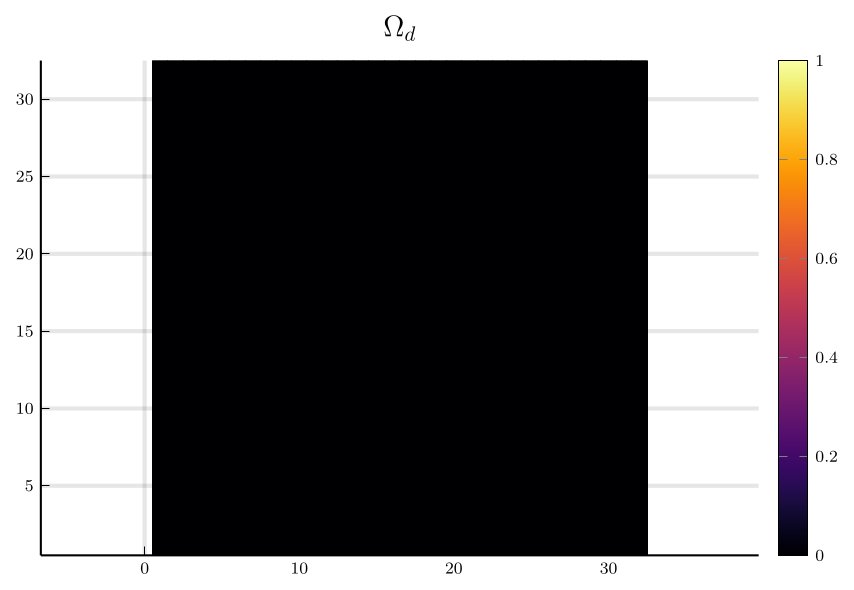
\includegraphics[width=.9\linewidth]{images/domain.png}
\label{}
\end{center}
\chapter{Numerical solver}
\label{sec:orgeeaed4d}
Contrary to the solver proposed in\autocite{Ulmer_CHRelaxed_2024} we do not use a multi-grid Gauss-Seidel Solver to solve the linear system, and use a Jacoby solver instead, since it is easier to paralyze.
Similar to \autocite{Ulmer_CHRelaxed_2024} we linearize \eqref{eq:second-order-adapted-ansatz} to
\begin{equation}
\begin{aligned}
\frac{\phi_{ij}^{n+1}}{\Delta t}  -  \nabla _d \cdot (G_{ij} \nabla_d \mu_{ij}^{n+\frac{1}{2}} ) &= \frac{ \phi_{ij}^n}{\Delta t}  \\
 \mu_{ij}^{n+\frac{1}{2}} - 2\phi_{ij}^{n+1} + \varepsilon^2  \nabla_d \cdot  (G_{ij} \nabla _d \phi_{ij}^{n+1} ) + B_{ij} &=2\phi _{ij}^n - W'(\phi_{ij}^n)
\end{aligned}
\end{equation}
After some rearranging we note, that the left-hand side is linear and, the right-hand side is solely dependent on the previous time step. Therefore, this constitutes a linear system, which we solve with a Jacoby method, the element wise formula of which is given as follows:
Provided the \(mth\) Jacoby iteration has been computed, the \(m+1th\) iteration is computed by solving
\begin{equation}
\begin{aligned}
\frac{\phi_{ij}^{n+1,m+1}}{\Delta t}  -  \nabla _d \cdot (G_{ij} \nabla_d \mu_{ij}^{n+\frac{1}{2},m+\frac{1}{2}} ) &= \frac{ \phi_{ij}^{n}}{\Delta t}  \\
 \mu_{ij}^{n+\frac{1}{2},m} - 2\phi_{ij}^{n+1,m} + \varepsilon^2  \nabla_d \cdot  (G_{ij} \nabla _d \phi_{ij}^{n+1,m+\frac{1}{2}} ) + B_{ij} &=2\phi _{ij}^n - W'(\phi_{ij}^n)
\end{aligned}
\end{equation}
For \(\phi_{ij}^{n+1,m+1} , \mu_{ij}^{n+\frac{1}{2},m+1}\),
where \(\nabla _d \cdot (G_{ij} \nabla_d \mu_{ij}^{n+\frac{1}{2},m+\frac{1}{2}} )\) and \(\nabla_d \cdot  (G_{ij} \nabla _d \phi_{ij}^{n+1,m+\frac{1}{2}} )\).  Use the results from the previous jacoby step for values off the center. eg.
\begin{equation}
\begin{aligned}
 \nabla _d \cdot (G_{ij} \nabla_d \phi_{ij}^{n+1,m+\frac{1}{2}} )  =&
\frac{1}{h^2} (
G_{i+\frac{1}{2}j}\phi_{i+1j}^{n+1,m}
+ G_{i-\frac{1}{2}j}\phi_{i-1j}^{n+1,m} \\
& + \quad G_{ij+\frac{1}{2}}\phi_{ij+1}^{n+1,m}
+ G_{ij-\frac{1}{2}}\phi_{ij-1}^{n+1,m}
 ) \\
& -
\left(
 G_{i+\frac{1}{2}j}
 + G_{i-\frac{1}{2}j}
 + G_{ij+\frac{1}{2}}
 + G_{ij-\frac{1}{2}}
\right)\phi_{ij}^{n+1,m+1}
\end{aligned}
\end{equation}
Our implementation makes use of the julia programming language, to dispatch the solution for each element in paralell on the GPU. The full implementation of the jacoby iteration is given as:
\begin{verbatim}
@kernel function jacoby!(
    Φ,
    M,
    @Const(Ξ),
    @Const(Ψ),
    @Const(h),
    @Const(ε),
    @Const(Δt),
    @Const(iterations)
)
    I   = @index(Global, Cartesian)
    Id  = oneunit(I)
    Ids = CartesianIndices(M)
    Ix = CartesianIndex(1, 0)
    Iy = CartesianIndex(0, 1)
    if I in (Ids[begin]+Id:Ids[end]-Id)
        g = G(2 * I + Ix, Ids) + G(2 * I + Iy, Ids) + G(2 * I - Ix, Ids) + G(2 * I - Iy, Ids)
        a1 = 1/Δt
        a2 = -1* ε^2/h^2 * g  - 2
        b1 = 1/h^2 * g
        b2 = 1
        for _ = 1:iterations

            Σμ = G(2 * I + Ix, Ids) * M[I+Ix] + G(2 * I + Iy, Ids) * M[I+Iy] + G(2 * I - Ix, Ids) * M[I-Ix] + G(2 * I - Iy, Ids) * M[I-Iy]

            Σϕ = G(2 * I + Ix, Ids) * Φ[I+Ix] + G(2 * I + Iy, Ids) * Φ[I+Iy] +G(2 * I - Ix, Ids) * Φ[I-Ix] +G(2 * I - Iy, Ids) * Φ[I-Iy]

            c1 = Ξ[I] + 1/h^2   * Σμ
            c2 = Ψ[I] - ε^2/h^2 * Σϕ

            # stupid matrix solve
            @inline Φ[I] = (c1*b2 - c2*b1) / (a1*b2 - a2*b1)
            @inline M[I] = (a1*c2 - a2*c1) / (a1*b2 - a2*b1)
            #
            @synchronize()
        end

    end
end
\end{verbatim}
\chapter{Numerical evaluation}
\label{sec:orgb47f456}
We set constant values for B\textsubscript{ij} on the boundary to begin with our evaluations.
One may note that C = 0 is equivalent to the no-flux condition of the original solver introduced in the Bachelor thesis. Now, as a preliminary verification step we set C = 0 as our first choice.
Consequently, for \(C = 0\), the interface lies orthogonal on the boundary (see Fig. \ref{fig:angle0}), which we expect for a CH solver with no-flux boundary conditions.
For \(B_{ij} \in \{-1,1\}\) we observed behavior connected to hydrophobic / hydrophilic substances on the boundary, where \(B_{ij}=1\) resulted in the one phase pearling off the boundary, while the other seemed attracted. These certainly leads to the apparent contact angles of 180° and 0° respectively. Using \(B_{ij} = -1\) results in the opposite behavior.


\begin{figure}[htbp]
\centering
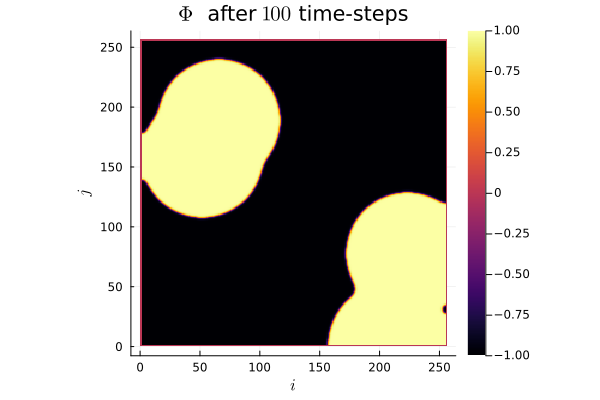
\includegraphics[width=.9\linewidth]{images/baseline.png}
\caption{\label{fig:angle0}phase-field \(\phi\) after 100 time-steps with \(C=0\) emmulating no-flux boundary.}
\end{figure}

We show, that our solver is stable for values \(C \neq 0\). In \ref{fig:angle1} we employ a constant value of \(C=1\) and observe the phase corresponding to \(\phi = 1\) puling away from the boundary. The contact angle between phase 1 and the boundary approaches 180° i.e. the interface runs parallel to the boundary.
\begin{figure}[htbp]
\centering
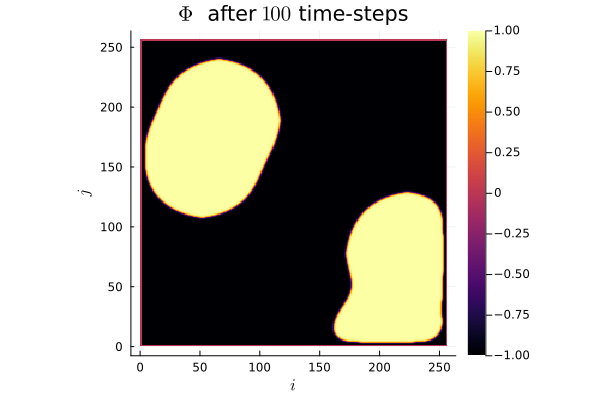
\includegraphics[width=.9\linewidth]{images/angle1.png}
\caption{\label{fig:angle1}phase-field   \(\phi\) after 100 time steps with \(C=1\)}
\end{figure}


In \ref{fig:angle-1} we try the reverse situation. And we observe corresponding behavior. When using a value of \(C=-1\) we observe opposite behavior relative to the case in Fig. \ref{fig:angle1}. Where the contact angle on the boundary lies at 0°, the interface runs parallel to the boundary again.
\begin{figure}[htbp]
\centering
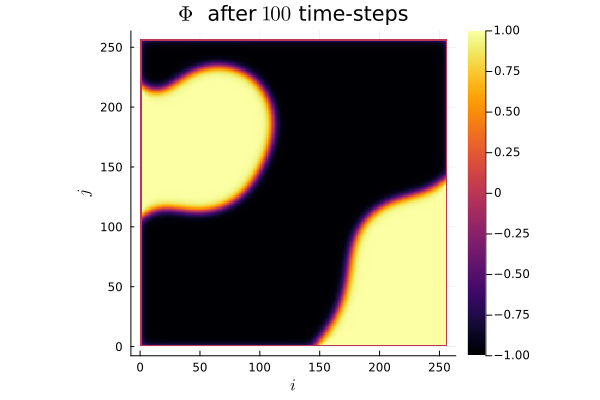
\includegraphics[width=.9\linewidth]{images/angle-.png}
\caption{\label{fig:angle-1}phase-field \(\phi\) after 100 time-steps with \(C=-1\)}
\end{figure}

The most interesting behavior are noted for values between \((-1,1)\), where we observe the contact angle of the interface at the boundary changes from parallel 0° to parallel 180°.
\begin{center}
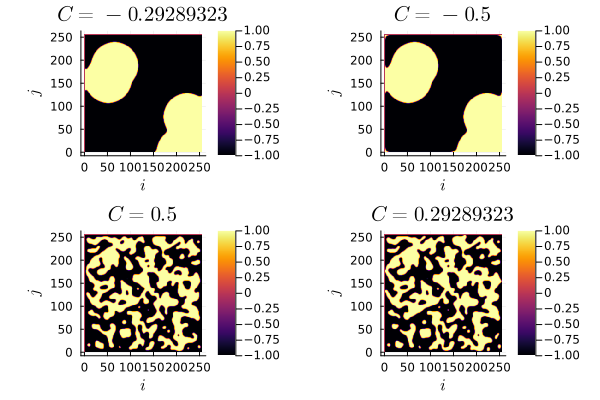
\includegraphics[width=.9\linewidth]{images/angle-sqrt(2).png}
\label{fig:angle-multiple}
\end{center}

\begin{verbatim}
include("src/solvers.jl")
θ = -5f-1
n = 100
arr = _init()
d = domain(get_backend(arr) , 256 , size(arr))
d(arr)
h = 25e-5
solution = solve(arr , n , θ=θ)
h1 = heatmap(Array(solution) , aspect_ratio=:equal , clims=(-1,1), lims=(0,size(solution,1)), widen=1.06 , title=L"h=%$h")
h = 20e-5
solution = solve(arr , n , θ=θ)
h2 = heatmap(Array(solution) , aspect_ratio=:equal , clims=(-1,1), lims=(0,size(solution,1)), widen=1.06 , title=L"h=%$h")
h = 15e-5
solution = solve(arr , n , θ=θ)
h3 = heatmap(Array(solution) , aspect_ratio=:equal , clims=(-1,1), lims=(0,size(solution,1)), widen=1.06 , title=L"h=%$h")
h = 10e-5
solution = solve(arr , n , θ=θ)
h4 = heatmap(Array(solution) , aspect_ratio=:equal , clims=(-1,1), lims=(0,size(solution,1)), widen=1.06 , title=L"h=%$h")
plot(h1,h2,h3,h4)
\end{verbatim}

\begin{center}
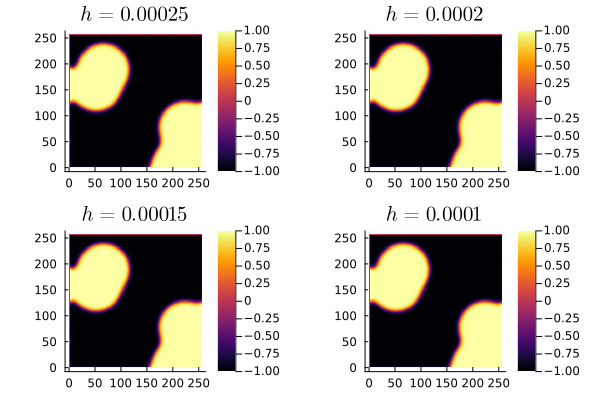
\includegraphics[width=.9\linewidth]{images/random-square.png}
\label{fig:random-square}
\end{center}
\chapter{Numerical evaluation on a circle}
\label{sec:org8f4cb79}
The original solver presented in \autocite{SHIN20117441} was able to solve the CH equation on arbitrary domains. Since the addition of our boundary function depends solely on the characteristic function of the discrete domain, we are able to use our approach on different Domains, by providing a different characteristic function. We present the results of which in this chapter.
To show the behavior of the CH solver in \ref{fig:angle0c}, we first employ no-flux boundary conditions on a circular domain. We observe the interface perpendicular on the boundary, as we expect.

\phantomsection
\label{}
\begin{verbatim}
W′ (generic function with 1 method)
\end{verbatim}



\begin{figure}[htbp]
\centering
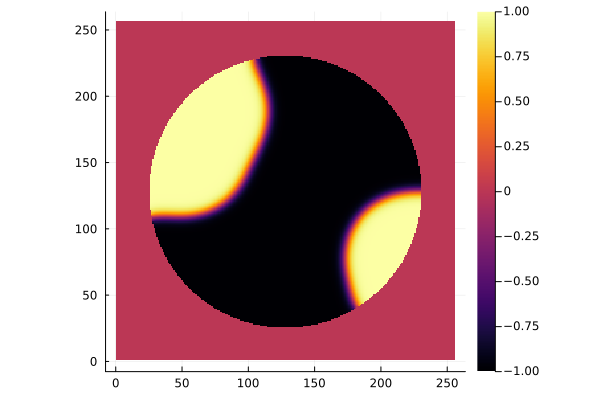
\includegraphics[width=.9\linewidth]{images/angle0c.png}
\caption{\label{fig:angle0c}\(\phi\) after 100 time steps on a circular domain with no-flux boundary-conditions after 100 time steps on a circular domain with no-flux}
\end{figure}



The results we observe in \ref{fig:angle1c} are similar to the results on a square domain in \ref{fig:angle1}. The contact angle is 180° i.e. the interface does not touch the boundary and runs parallel to it.
\begin{figure}[htbp]
\centering
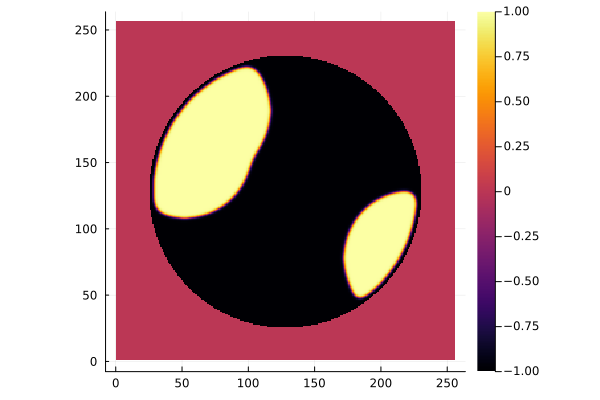
\includegraphics[width=.9\linewidth]{images/anfle1c.png}
\caption{\label{fig:angle1c}phase-field \(\phi\) after 100 time-steps with \(C=1\)}
\end{figure}

The results for \(C=-1\) in \ref{fig:angle-1c} on the circular domain, are similar to the results in \ref{fig:angle-1} on the square domain as well, where the interface touches the boundary and runs parallel with a contact angle of 0°.
\begin{figure}[htbp]
\centering
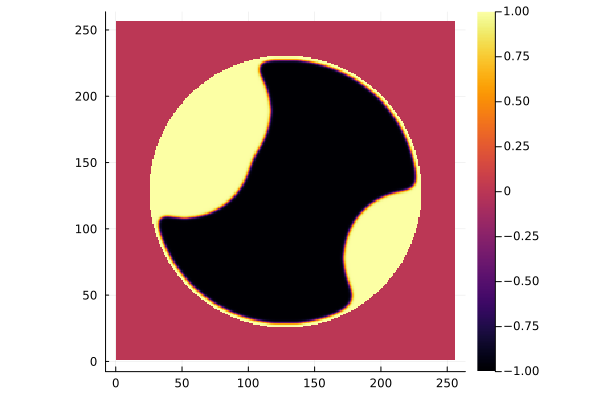
\includegraphics[width=.9\linewidth]{images/angle-1c.png}
\caption{\label{fig:angle-1c}phase-field \(\phi\) after 100 time-steps with \(C=-1\)}
\end{figure}

When evaluating intermediate contact angles in \ref{fig:angle-multiplec}, the results are similar to the square domain again, however, especially for shallow angles, we observe some artifacts of one phase appearing in places where previously was none. We observe similar behavior on square domains only in the corners, i.e. points where the boundary has high curvature.
\begin{figure}[htbp]
\centering
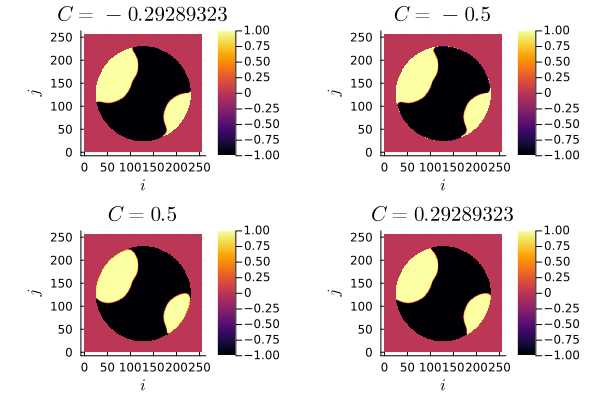
\includegraphics[width=.9\linewidth]{images/angle-multiplec.png}
\caption{\label{fig:angle-multiplec}phase-field \(\phi\) after 500 time-steps with \(C \in \{-1 + \frac{\sqrt{2}}{2} , -0.5 , 0.5 , 1 - \frac{\sqrt{2}}{2} \}\) on a circular domain.}
\end{figure}



When using random initial phase-fields, the results look the comparable to the square domain, and exhibit the for the CH equation expected behavior, whereas time goes on, the many small parts coalesce into larger parts.
\chapter{angle}
\label{sec:org214e230}
In previous experiments we noted that the angle of the interface changes with different input parameters. While we do not have a mathematical derivation of this relation, we aim to provide numerical insight in this chapter. We calculate this angle using the gradient of the phase-field \(\nabla \phi_{ij}\) and the normal of our domains' boundary.
\begin{align}
\label{eq:1}
\frac{\nabla_d \phi_{ij} \cdot \mathbf{n}_{ij}}{\|\nabla_{d} \phi_{ij}\|} &= \cos(\theta)& & \phi_{ij} \in \partial\Omega_{d}
\end{align}
For a single point \(\vec{x}_{ij}\) on the interface and near the boundary. Since we need a finite difference to evaluate \ref{eq:1}, we do not select a point directly on the boundary and since we need a point on the interface, where \(\nabla \phi_{ij}\) is large, we calculate the angle at
\begin{equation}
\label{eq:2}
P_{ij} = arg\max_{\vec{x}_{ij}} \nabla \phi_{ij} \qquad \phi_{ij} \in \partial \Omega
\end{equation}
\phantomsection
\label{angle-function}
\begin{verbatim}
angle (generic function with 1 method)
\end{verbatim}
\section{circle}
\label{sec:org7d89b0f}
The normal the circular domain in our second example is
\begin{equation}
\label{eq:3}
\mathbf{n}_{ij} := \mathbf{n}(\vec{x}_{ij}) = \frac{\vec{c} - \vec{x}_{ij}}{\| \vec{c} - \vec{x}_{ij}\|}
\end{equation}
Where \(\vec{c}\) is the center of the domain.
\begin{center}
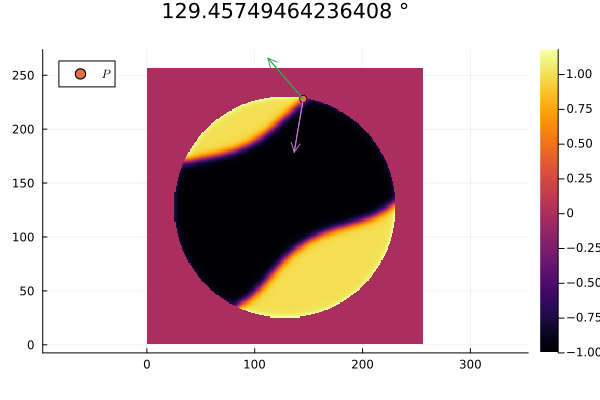
\includegraphics[width=.9\linewidth]{images/angle.png}
\label{angle-on-circle}
\end{center}

\begin{center}
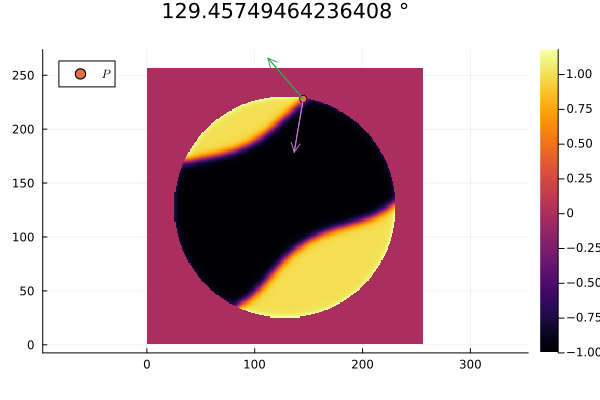
\includegraphics[width=.9\linewidth]{images/angle.png}
\label{angle-evaluation}
\end{center}


\begin{longtable}{rr}
\caption{\label{angle-table}value for \(\theta\) and corresponding angle \(\alpha\) after 200 time-steps}
\\
-0.1 & 173.49096591056502\\
-0.095 & 173.10715739345923\\
-0.09 & 172.18364087939332\\
-0.085 & 171.54740091859054\\
-0.08 & 171.3054040677464\\
-0.075 & 171.1455632002332\\
-0.07 & 171.02869693204397\\
-0.065 & 170.3901810227686\\
-0.06 & 170.0449796355949\\
-0.055 & 173.27274052589075\\
-0.05 & 170.3373892767722\\
-0.045 & 168.11953739721892\\
-0.04 & 167.41386769034298\\
-0.035 & 166.62088559081457\\
-0.03 & 164.9014365935728\\
-0.025 & 162.8061312020723\\
-0.02 & 159.92337650959868\\
-0.015 & 155.82320048245077\\
-0.01 & 147.4707481361878\\
-0.005 & 129.77836444929315\\
0.0 & 91.28977210940522\\
0.005 & 47.27538237804684\\
0.01 & 26.60911004838421\\
0.015 & 6.306468865037136\\
0.02 & 11.495581754132852\\
0.025 & 8.059259459078769\\
0.03 & 2.997826637980469\\
0.035 & 2.442790881259583\\
0.04 & 2.314200756133827\\
0.045 & 1.883610279597664\\
0.05 & 1.3567468712125557\\
0.055 & 0.8024311153759808\\
0.06 & 0.5869880299417852\\
0.065 & 0.4356076759230446\\
0.07 & 0.32719257485287145\\
0.075 & 0.03099970458170946\\
0.08 & 0.37685133141547533\\
0.085 & 0.4151229191583983\\
0.09 & 0.7049376111739059\\
0.095 & 0.8671639875701463\\
0.1 & 1.0282690721714873\\
\end{longtable}
\chapter{Summary and outlook}
\label{sec:org0664668}
In this project we examined a numerical model o the CH equation, with simple Neumann boundary conditions. We introduced a simplified version of the solver used in \autocite{Ulmer_CHRelaxed_2024} and derived from \autocite{SHIN20117441}. Which due to GPU acceleration is significantly faster on our available hardware. We have shown a simple Neumann boundary approach that runs stable on both tested domains. The approach introduced by us is able to freely affect the angle of the phase interface on the boundary,
\chapter{References}
\label{sec:org34e895a}
\printbibliography
\end{document}
